%%%%%%%%%%%%%%%%%%%%%%%%%%%%%%%%%%%%%%
%%%%%%%%%%%%%%%%%%%%%%%%%%%%%%%%%%%%%%
% Do not edit the TeX file your work
% will be overwritten.  Edit the RnW
% file instead.
%%%%%%%%%%%%%%%%%%%%%%%%%%%%%%%%%%%%%%
%%%%%%%%%%%%%%%%%%%%%%%%%%%%%%%%%%%%%%





\newcommand{\DefineMacros}{
\begin{kframe}


{\ttfamily\noindent\bfseries\color{errorcolor}{\#\# Error in `prettyNum()`:\\\#\# ! invalid value 0 for 'digits' argument}}\end{kframe}
}

%%%%%%%%%%%%%%%%%%%%%%
%%%%%%%%%%%%%%%%%%%%%%
%%%%%%%%%%%%%%%%%%%%%%
% Tables

\newcommand{\CashTransfersResultsTable}{
% \input{figures/cash_transfers_re_run_table.tex}
\begin{kframe}


{\ttfamily\noindent\bfseries\color{errorcolor}{\#\# Error in `pivot\_wider()`:\\\#\# ! `id\_cols` can't select a column already selected by `names\_from`.\\\#\# i Column `metric` has already been selected.}}\end{kframe}
}

%%%%%%%%%%%%%%%%%%%
% OHIE

\newcommand{\OHIEResultsTable}{
% \input{figures/OHIE_table_9_IV_re_run_table.tex}


\begin{table}\small 
\begin{tabular}{|ccc|}
\toprule
 Original estimate (SE) & Refit estimate (SE)  & Observations dropped \\
\midrule
\midrule
\begin{kframe}

{\ttfamily\noindent\bfseries\color{errorcolor}{\#\# Error in `pivot\_wider()`:\\\#\# ! `id\_cols` can't select a column already selected by `names\_from`.\\\#\# i Column `metric` has already been selected.}}\end{kframe}
}


%%%%%%%%%%%%%%%%%%%
% Microcredit
%
\newcommand{\MicrocreditProfitResultsTable}{
% \input{figures/microcredit_profit_re_run_table.tex}
\begin{kframe}


{\ttfamily\noindent\bfseries\color{errorcolor}{\#\# Error in `pivot\_wider()`:\\\#\# ! `id\_cols` can't select a column already selected by `names\_from`.\\\#\# i Column `metric` has already been selected.}}\end{kframe}
}
%
%
% \newcommand{\MicrocreditTemptationResultsTable}{
% % \input{figures/microcredit_profit_re_run_table.tex}
% <<microcredit_temptation_results_table, cache=microcredit_cache, results='asis'>>=
% source("figures_knitr/microcredit/microcredit_temptation_results_table.R",
%        echo=knitr_debug, print.eval=TRUE)
% @
% }

%%%%%%%%%%%%%%%%%%%
% Microcredit mixture
%
% \newcommand{\MicrocreditMixtureResultsTable}{
% <<mcmix_re_run_table, cache=mcmix_cache, results='asis'>>=
% source("figures_knitr/microcredit_mixture/microcredit_mix_refit_table.R",
%        echo=knitr_debug, print.eval=TRUE)
% @
% }
%
% \newcommand{\MicrocreditMixtureSdResultsTable}{
% <<mcmix_sd_re_run_table, cache=mcmix_cache, results='asis'>>=
% source("figures_knitr/microcredit_mixture/microcredit_mix_sd_refit_table.R",
%        echo=knitr_debug, print.eval=TRUE)
% @
% }

%%%%%%%%%%%%%%%%%%%%%%
%%%%%%%%%%%%%%%%%%%%%%
%%%%%%%%%%%%%%%%%%%%%%
% Graphs


\newcommand{\SimInflHistogram}{

\begin{knitrout}
\definecolor{shadecolor}{rgb}{0.969, 0.969, 0.969}\color{fgcolor}

{\centering 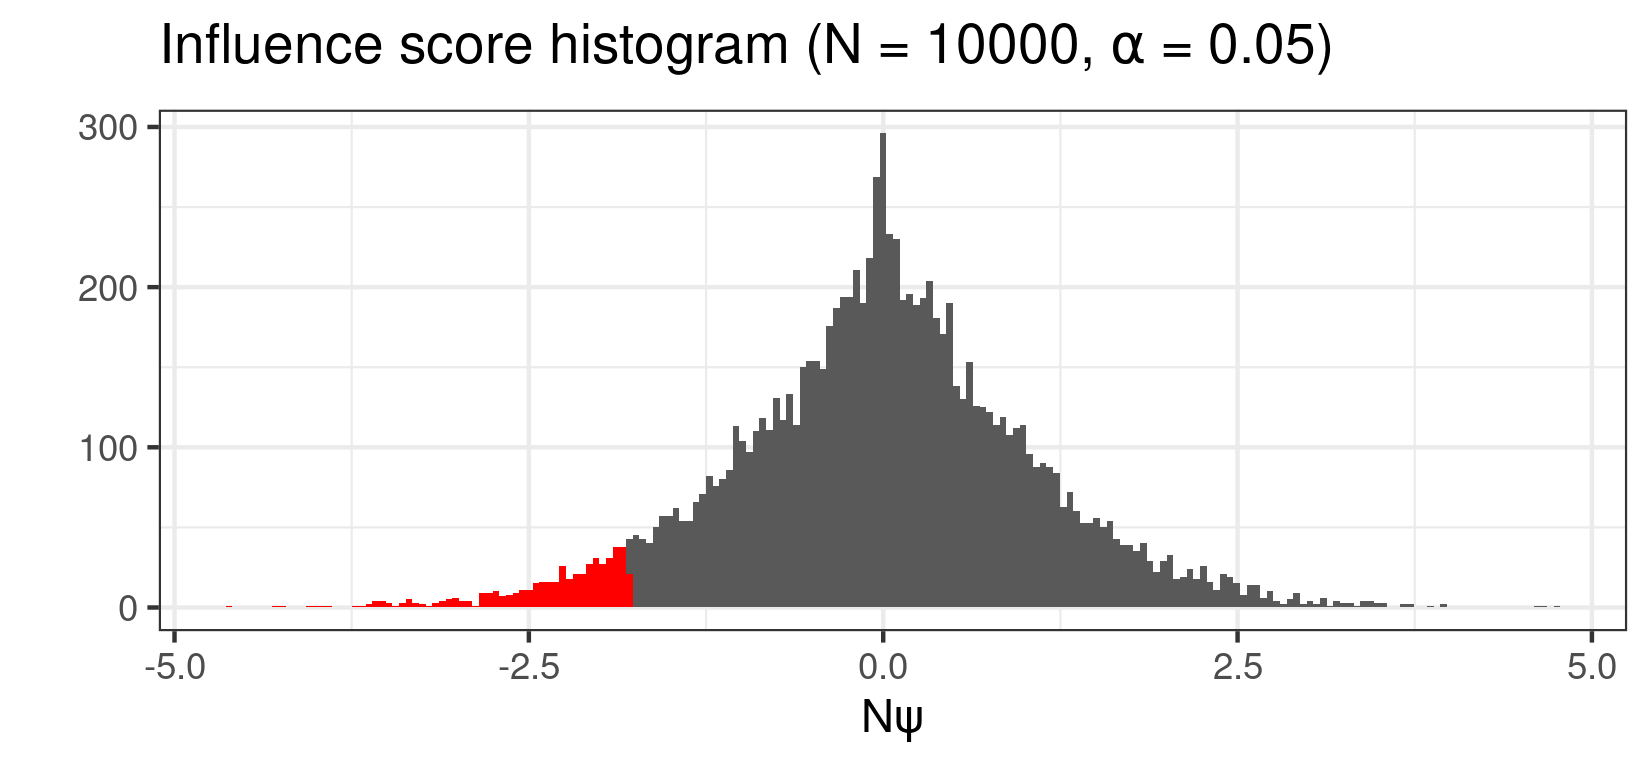
\includegraphics[width=0.98\linewidth,height=0.461\linewidth]{figure/sim-infl-hist-1} 

}


\end{knitrout}
}





\newcommand{\SimRefitOne}{
\begin{knitrout}
\definecolor{shadecolor}{rgb}{0.969, 0.969, 0.969}\color{fgcolor}

{\centering 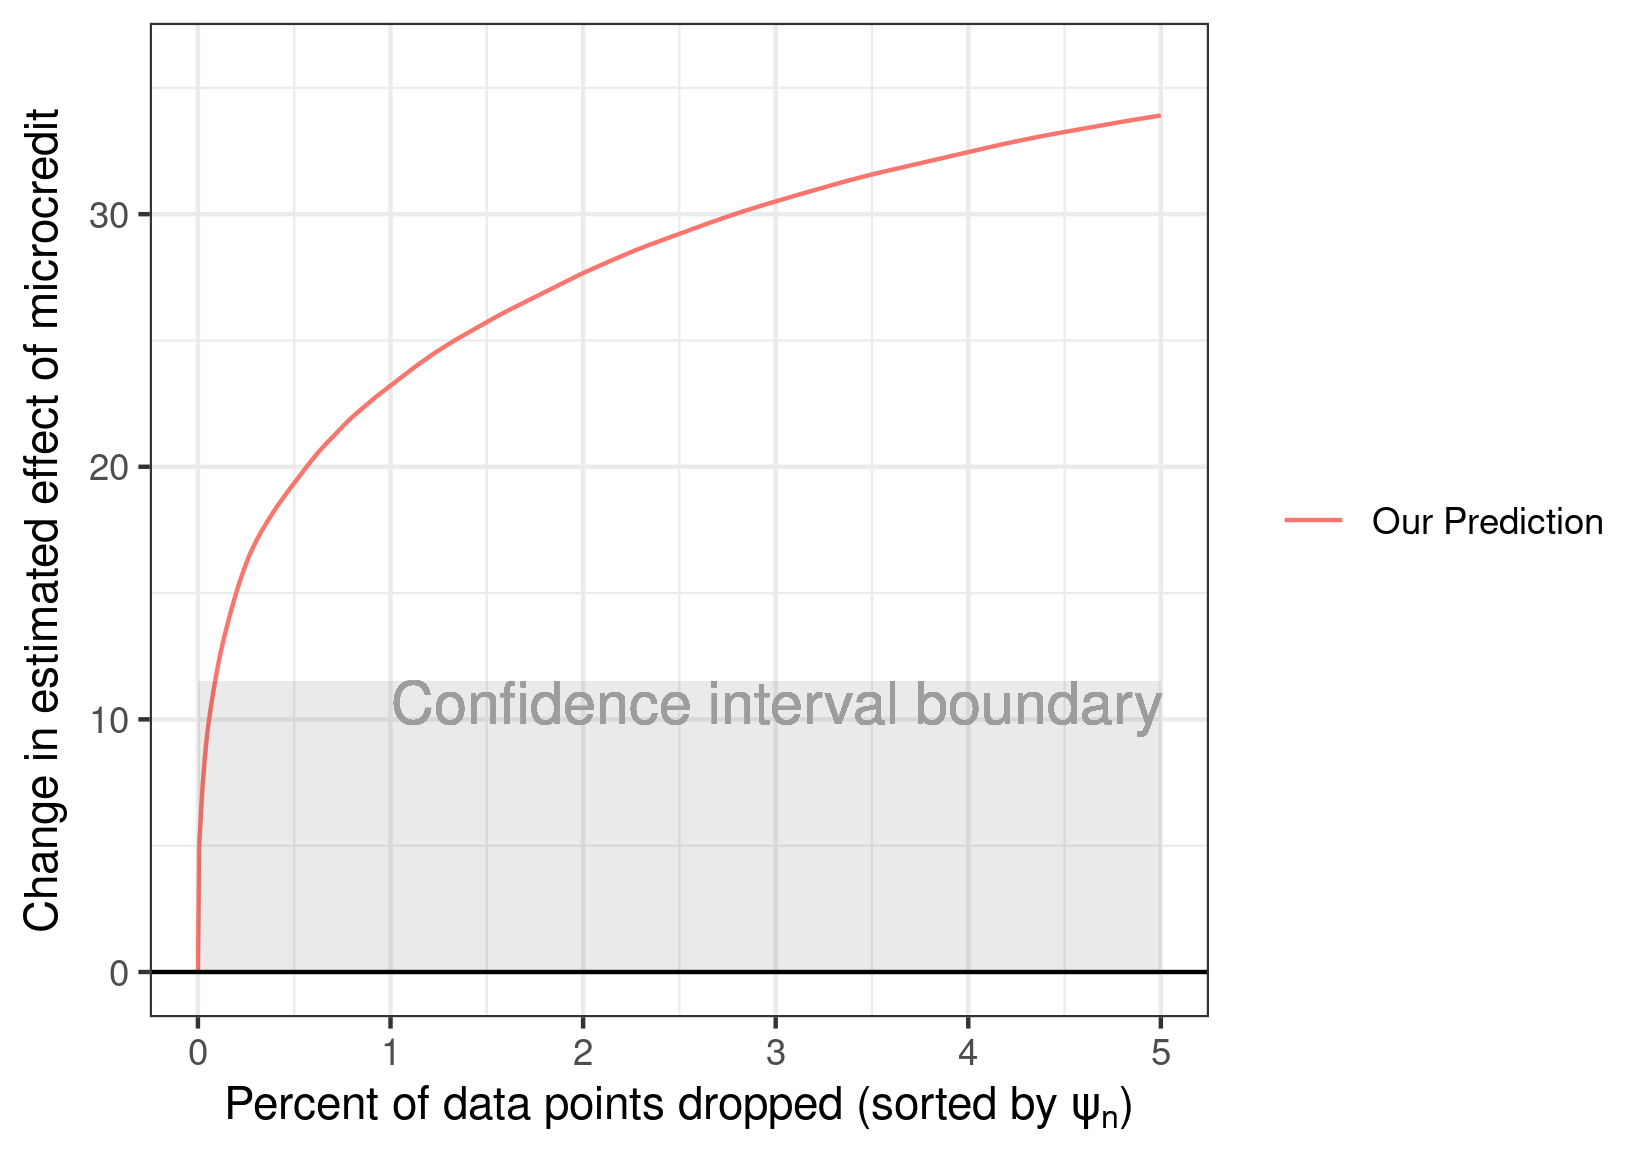
\includegraphics[width=0.98\linewidth,height=0.692\linewidth]{figure/sim-refit-one-1} 

}


\end{knitrout}
}

\newcommand{\SimRefitTwo}{
\begin{knitrout}
\definecolor{shadecolor}{rgb}{0.969, 0.969, 0.969}\color{fgcolor}

{\centering 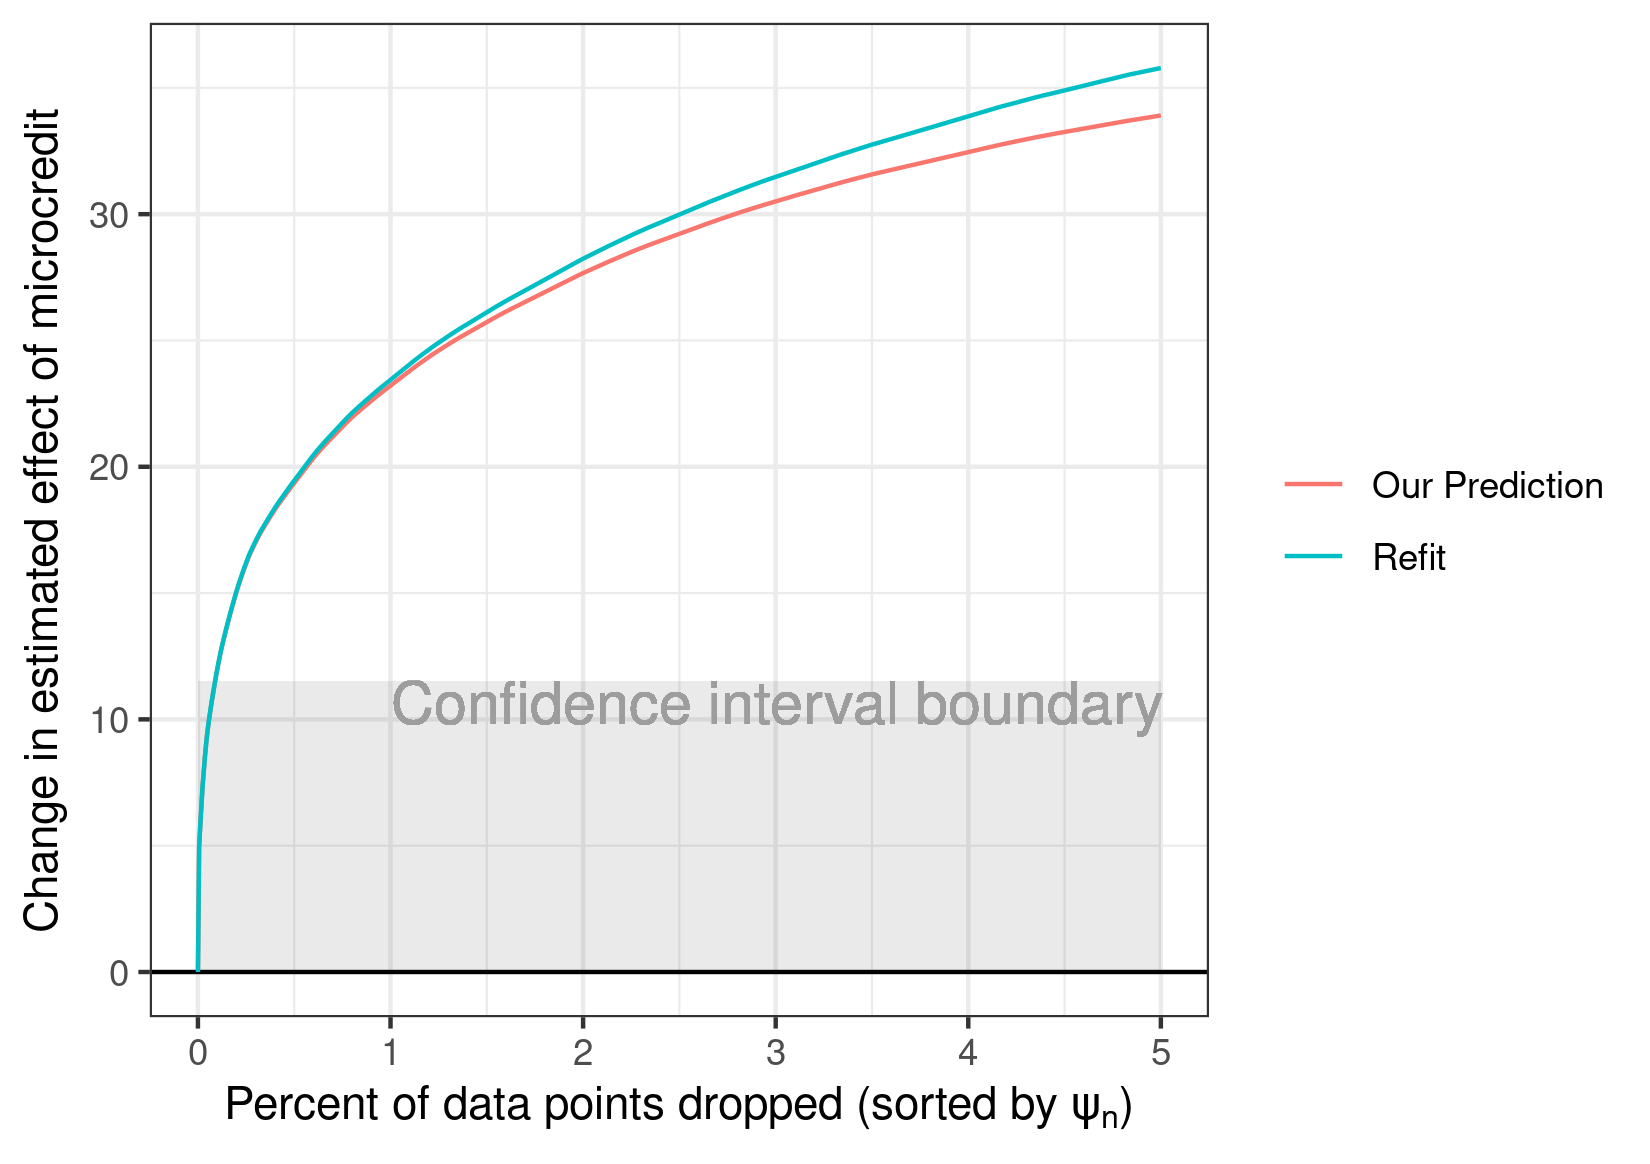
\includegraphics[width=0.98\linewidth,height=0.692\linewidth]{figure/sim-refit-two-1} 

}


\end{knitrout}
}



\newcommand{\SimApproxNormalGraph}{

\begin{knitrout}
\definecolor{shadecolor}{rgb}{0.969, 0.969, 0.969}\color{fgcolor}\begin{figure}[!h]

{\centering 
\includegraphics[width=0.98\linewidth,height=0.461\linewidth]{figure/sim-approx-normal-1} 

}

\caption[The actual change, linear approximation to the change, and approximation error.Here, $\sigma_x = \SimAccSigx$, $\sigma_\varepsilon = \SimAccSigeps$, and $\theta_0 = \SimTrueTheta$]{The actual change, linear approximation to the change, and approximation error.Here, $\sigma_x = \SimAccSigx$, $\sigma_\varepsilon = \SimAccSigeps$, and $\theta_0 = \SimTrueTheta$.}\label{fig:sim-approx-normal}
\end{figure}

\end{knitrout}
}

\newcommand{\SimGridNormalGraph}{

\begin{knitrout}
\definecolor{shadecolor}{rgb}{0.969, 0.969, 0.969}\color{fgcolor}\begin{figure}[!h]

{\centering 
\includegraphics[width=0.98\linewidth,height=0.384\linewidth]{figure/sim-grid-normal-1} 

}

\caption[The approximate perturbation inducing proportion at differing values of $\sigma_x$ and $\sigma_\varepsilon$]{The approximate perturbation inducing proportion at differing values of $\sigma_x$ and $\sigma_\varepsilon$. Red colors indicate datasets whose sign can is predicted to change when dropping less than 1\% of datapoints. The grey areas indicate $\amip{\alpha} = \na$, a failure of the linear approximation to locate any way to change the sign.}\label{fig:sim-grid-normal}
\end{figure}

\end{knitrout}
}



\newcommand{\MxProfitHistogram}{

\begin{knitrout}
\definecolor{shadecolor}{rgb}{0.969, 0.969, 0.969}\color{fgcolor}

{\centering 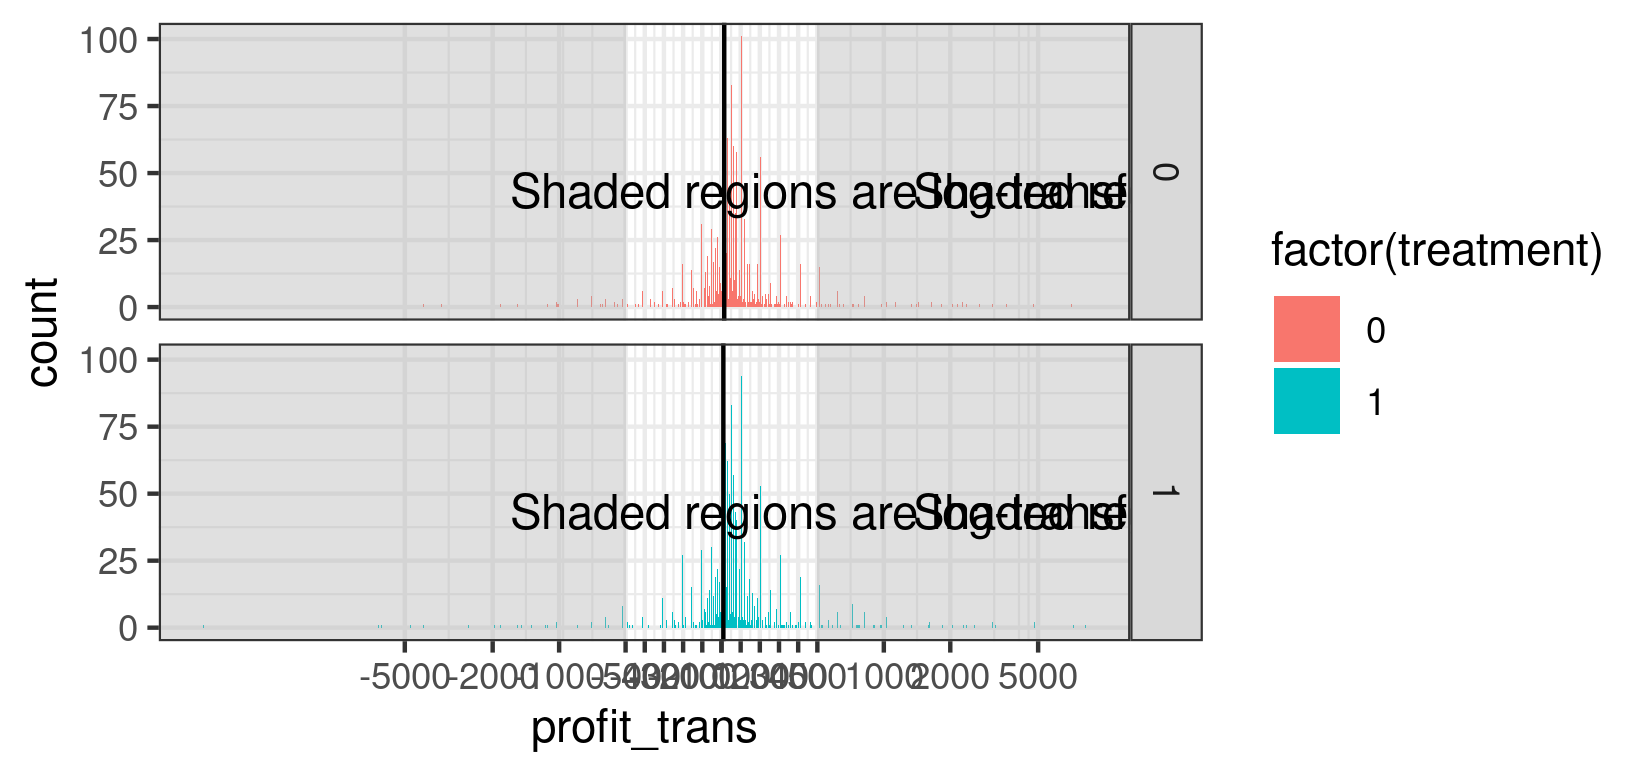
\includegraphics[width=0.98\linewidth,height=0.461\linewidth]{figure/mx-hist-1} 

}


\end{knitrout}
}
